\documentclass[10pt]{article}

% Default 
\usepackage{graphicx}
\usepackage[backend=biber,
  style=numeric, 
  sorting=none]{biblatex}

% Additional
\usepackage{amsmath}
\usepackage{textcomp, gensymb}
\usepackage{placeins}
\usepackage{tabularray} 
\usepackage{xcolor}
\usepackage{placeins}
\usepackage{csquotes} 
\usepackage{todonotes}
\usepackage{hyperref}
\usepackage{siunitx}

\newcommand{\td}[1]{\todo[linecolor=blue, backgroundcolor=blue!25,bordercolor=blue, size=\small, inline]{#1}}

\addbibresource{references.bib}

\title{Michelson Interferometer} 
\author{Rahmanyaz Annyyev, Hikmat Gulaliyev}
\date{28 April, 2024} 

\begin{document}

\maketitle

\begin{abstract}
  In this experiment, the Michelson interferometer was used to dive into the concept of wave interference. The interferometer splits a laser beam into two coherent beams and later recombines them after reflecting from mirrors to create an interference pattern on the screen. By adjusting one of the mirrors, we can change the path of one beam, and therefore observe variations in the pattern as destructive and constructive interferences occur.

  The experiment consists of two parts where first one focuses on measuring the wavelength of laser light. This was achieved by counting the number of fringe cycles as the mirror position changed precisely, which in combination with the known relationship between phase shift and path difference allows for accurate results.
  
  The second part of the experiment was dedicated to measuring the refractive index of air. By adding a variable-pressure vacuum chamber to the setup, we can mimic the role of the change in the optical path we gained from mirror movement in the previous part. Similarly, by observing fringe cycles, we can find the refractive index of air. 

  The results of the experiment were found to be in good agreement with the theoretical values, although fringe patterns weren't perfectly circular and fully observable.
\end{abstract}

\section{Introduction}

\subsection*{General}

One of the methods of producing interference patterns is amplitude division. In this method, a beam of light is divided into two beams, and the two beams are recombined to produce interference fringes. A Michelson interferometer is an instrument that employs this mechanism.

A Michelson interferometer is an instrument used in optical interferometry. Minimally, it consists of two mirrors $M_1$ and $M_2$ and a beam splitter $M$ (although a diffraction grating can be used). The setup is shown in Figure \ref{fig:1}. The beam splitter, in our case, is a plate beamsplitter with a partially reflective coating. A source of light, $S$, a laser in our case, is directed at the beam splitter, and the light is split into two beams of coherent light at point $C$. One beam is reflected toward fixed mirror $M_1$, and the other one is transmitted toward adjustable mirror $M_2$. The beams are reflected by the mirrors and recombined at the beam splitter at point $C'$. They then travel to a viewing screen where the interference pattern is observed (although a photoelectric detector or a camera can be used) \cite{Hecht_2017}.

\begin{figure}[hbt!]
  \centering
  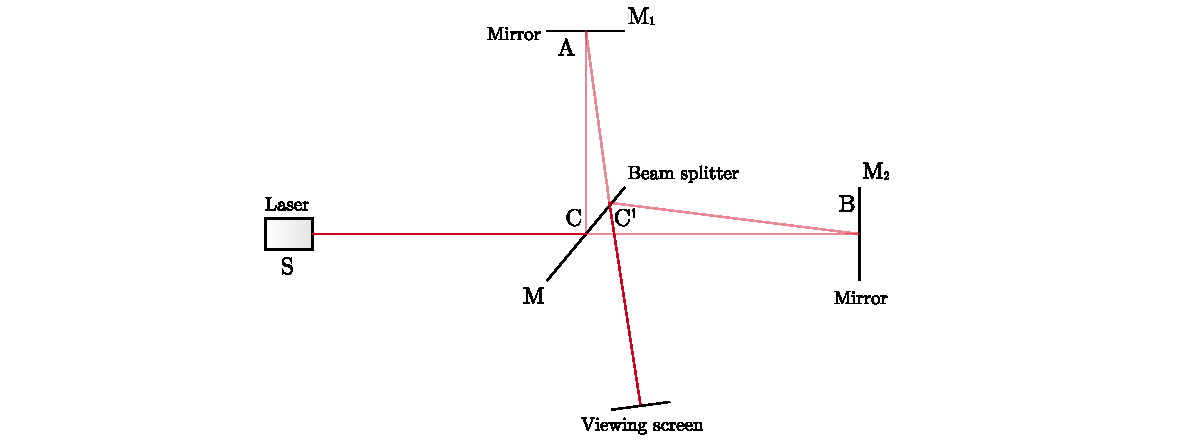
\includegraphics[scale=0.6]{figures/f1.pdf}
  \caption{The Michelson interferometer.}
  \label{fig:1}
\end{figure}

The beam of light that is produced by a He-Ne laser is too narrow for us to observe the interference fringes. To widen the beam, we use a lens, $L$, which is placed between the beam splitter and the screen. It spreads the beam, and the interference fringes become visible. However, only the central ray of the beam travels in a straight line. The rays that are further from the center travel at an angle and, therefore, have a different path length. This difference in path length causes the interference fringes to be curved. To make the fringes straight, we place the mirrors $M_1$ and $M_2$ at an angle of $90\degree$ to each other. This way, the rays that are reflected by the mirrors travel the same distance and the fringes are straight. 

The interference pattern will be a series of bright and dark concentric rings. The rings are formed because, as we stated earlier, as the rays are reflected by the mirrors, they travel different distances, and hence, have different relative phases. The relative phase difference includes the changes in phase due to the reflection of the light from the mirrors and the difference in the total path length the light travels. 

In this experiment, we are concerned with the phase changes. We can calculate the number of cycles of fringes that are produced as the mirror $M_2$ is moved. The amount of phase change is given by the formula
\begin{equation}
  \Delta \phi = 2 \pi \left(\dfrac{d}{\lambda/n}\right) = 2 \pi n \left(\dfrac{d}{\lambda}\right)
  \label{eq:1}
\end{equation}
where $d$ is the distance the mirror is moved, $\lambda$ is the wavelength of the light in a vacuum, and $n$ is the refractive index of the medium in which the light is traveling \cite{Pedrotti_2006}. Therefore, the interference pattern switches from bright to dark $N$ times as the mirror is moved a distance $d$ given by
\begin{equation}
  N \lambda = 2 n d
  \label{eq:2}
\end{equation}

\subsection*{Procedure}

The experiment is comprised of two parts: A and B. The setup consists of a PASCO{\textsuperscript\textregistered} interferometer, a lens with a holder, a viewing screen, a vacuum pump, a He-Ne laser, and a vacuum chamber.

\subsubsection*{Part A}

In the first part of the experiment, we will measure the wavelength of the light produced by the He-Ne laser. We will count the number of fringes, $N$, that pass a point on the screen as the mirror $M_2$ is moved a distance $d$. We will then use Equation (\ref{eq:2}) to calculate the wavelength of the light. Since $N$ can be quite large for a coherent light source like a laser, the precision of the measurement can be quite high. 

We first adjust the interferometer and the laser until a nearly circular, or elliptical, pattern is observed on the screen. Next, we adjust the micrometer knob so that the lever arm is nearly parallel with the edge of the interferometer base. In such a case, the relationship between the rotation of the knob and the movement of the mirror is almost linear. We turn the micrometer knob one full turn counterclockwise until the zero mark on the knob is aligned with the index mark. Next, we select a mark on the screen, slowly turn the micrometer counterclockwise, and observe the change in the interference pattern. Then, we count the number of fringes that pass the mark on the screen as we turn the knob. The final position of the knob and the distance $d$ the mirror has moved are recorded. At least 30 fringes should be counted, and the measurement should be repeated at least four times to obtain appreciable accuracy. All of the measurements should be recorded in a table.

\subsubsection*{Part B}

In the second part of the experiment, we will measure the refractive index of air. First, we align the laser and the interferometer just as we did in the first part of the experiment. Next, we fix the mirrors and place a vacuum chamber between the mirror $M_2$ and the beam splitter. The end plates of the vacuum chamber must be perpendicular to the axis of the interferometer for the best results. Then, we adjust the alignment screws of the mirror $M_1$ so that the center of the interference pattern is observed on the screen. We make a mark on the screen and evacuate the chamber.

As the air is pumped out of the chamber, the refractive index of the air will decrease, and the interference pattern will shift on the viewing screen. By counting the number of fringes that pass a point on the screen for different values of $P_{\text{final}}$, we can calculate the refractive index of the air using the formula
\begin{equation}
  n_{\text{atm}} = 1 + \dfrac{\lambda}{2d} \dfrac{N}{\Delta P} P_{\text{atm}}
\end{equation}
where $n_{\text{atm}}$ is the refractive index of the air at atmospheric pressure, $N$ is the number of fringes that pass a point on the screen, $\Delta P$ is the change in pressure within the chamber, $P_{\text{atm}}$ is the atmospheric pressure, $\lambda$ is the wavelength of the light in vacuum, and $d$ is the thickness of the chamber. As an assumption, the temperature of the air is kept constant. 

\section{Data \& Results}

\subsection*{Part A}

The data obtained in the first part of the experiment is shown in Table (\ref{tab:1}). The average wavelength of the light produced by the He-Ne laser is calculated using Equation (\ref{eq:1}). It is assumed that the refractive index of air is $n = 1$. The average wavelength is calculated using the formula
\begin{equation}
  \bar{\lambda} = \dfrac{\sum_{i=1}^{n} \lambda_i}{n}
  \label{eq:3}
\end{equation}
and the standard deviation of the wavelength is calculated using the formula
\begin{equation}
  \Delta \lambda = \sqrt{\dfrac{\sum_{i=1}^{n} \left(\lambda_i - \bar{\lambda}\right)^2}{n-1}}
  \label{eq:4}
\end{equation}
where $n$ is the number of measurements. The wavelength of the light produced by the He-Ne laser is found to be $\lambda = \bar{\lambda} \pm \Delta \lambda$ nm.

\begin{table}[ht]
  \centering
  \vspace{4mm}
  \begin{tblr}{
    cells = {halign = c, valign = m},
    row{odd} = {bg = lightgray!5},
    row{1, 7} = {bg = lightgray!20},
    hlines = {},
    vlines = {}
  }
    $d_i$ (\si{\micro\metre}) & $N_i$ & $\lambda_i$ (nm) \\
    \hline 
    12 & 35 & 685.7 \\
    10.5 & 31 & 677.4 \\
    10 & 30 & 666.7 \\
    8.5 & 25 & 680.0 \\
    8 & 24 & 666.7 \\
    \hline
    $\bar{\lambda}$ (nm) & $\Delta \lambda$ (nm) & $\lambda$ (nm) \\
    675.3 & 8.4 & 675.3 $\pm$ 8.4
    
  \end{tblr}
  \caption{Results of the first part of the experiment.}
  \label{tab:1}
\end{table}

The value of the wavelength of the light produced by the He-Ne laser is found to be $\lambda = 675.3 \pm 8.4$ nm. The value is not in agreement with the accepted value of the wavelength of the light produced by a He-Ne laser, which is $\lambda = 632.8$ nm. The discrepancy could be due to errors in the measurements, the assumptions made in the calculations, or the approximations made in the experiment.

\td{Questions 4 and 5.}

\subsection*{Part B}

The data obtained in the second part of the experiment is shown in Table (\ref{tab:2}). The refractive index of air is calculated using Equation (\ref{eq:2}). The thickness of the chamber was found to be $3.3$ cm. The average refractive index of air is calculated using the formula
\begin{equation}
  \bar{n}_{\text{air}} = \dfrac{\sum_{i=1}^{n} n_{\text{air}_i}}{n}
  \label{eq:5}
\end{equation}
and the standard deviation of the refractive index is calculated using the formula
\begin{equation}
  \Delta n_{\text{air}} = \sqrt{\dfrac{\sum_{i=1}^{n} \left(n_{\text{air}_i} - \bar{n}_{\text{air}}\right)^2}{n-1}}
  \label{eq:6}
\end{equation}
where $n$ is the number of measurements. The refractive index of air is found to be $n_{\text{air}} = \bar{n}_{\text{air}} \pm \Delta n_{\text{air}}$.

\begin{table}[ht]
  \centering
  \vspace{4mm}
  \begin{tblr}{
    cells = {halign = c, valign = m},
    row{odd} = {bg = lightgray!5},
    row{1, 4} = {bg = lightgray!20},
    hlines = {},
    vlines = {}
  }
    $\Delta P_i$ (cmHg) & $N_i$ & $n_{\text{air}_i}$ \\
    \hline 
    20 & 10 & 1.00036 \\
    16 & 13 & 1.00059 \\
    \hline
    $\bar{n}_{\text{air}}$ & $\Delta n_{\text{air}}$ & $n_{\text{air}}$ \\
    1.00048 & 0.00016 & 1.00048 $\pm$ 0.00016
    
  \end{tblr}
  \caption{Results of the second part of the experiment.}
  \label{tab:2}
\end{table}

According to Mathar (2007), the refractive index of air is $n = 1.00027270$, which indicates that the measurement we obtained is ever so slightly higher than the actual value \cite{Mathar_2007}. The discrepancy could be due to errors in the measurements, the assumptions made in the calculations, or the approximations made in the experiment. 

\td{Question 3.}

\section{Discussion \& Conclusion}

\subsection*{Errors}

The sources of error in this experiment include alignment error, human error, imperfect instrumentation, and external factors.

\begin{itemize}
  \item \textbf{Alignment error:} The lens, mirrors, and the beam splitter may not have been perfectly aligned, which could have caused the interference pattern to be distorted. 
  \item \textbf{Human error:} The measurements of the number of fringes that pass a point on the screen may not be accurate since the fringes were counted manually. 
  \item \textbf{Imperfect instrumentation:} The beam splitter may have not split the light evenly and the lens may have not been perfectly transparent, which could have affected the interference pattern. The mirrors may not have been perfectly reflective, which could have caused the light to be absorbed or scattered.
  \item \textbf{External factors:} The temperature of the air in the chamber may not have been constant, which could have affected the refractive index of the air. Vibrations, air currents, and other external factors could have affected the path length of the light, leading to phase shifts and errors in the measurements. 
\end{itemize}

\subsection*{Approximations}
\begin{itemize}

\item \textbf{Refractive index of air:} The refractive index of air was assumed to be $n = 1$ in the calculations for part A.

\item \textbf{Temperature of the air:} The temperature of the air in the chamber was assumed to be constant. 

\item \textbf{Coherence of light:} It is assumed that the light is always coherent, and 

\item \textbf{Homogeneity of the medium:} It is assumed that the medium in which the light propagates is homogeneous and isotropic.

\item \textbf{Reflection of light:} It is assumed that the reflection of light from the mirrors is perfect and that no light is absorbed or scattered.

\end{itemize}

\subsection*{Discrepancies}

The discrepancies found in part A of the experiment for the values of the wavelength of the light can be explained by above mentioned errors and approximations. Difference between the measured and accepted values of the wavelength is around 7\%, which doesn't fall within the error margin of the experiment. The discrepancies found in part B of the experiment for the values of the refractive index of air can be explained by the same reasons. Measured value however is in great agreement with the theoretical value. 
\subsection*{Conclusion}

In conclusion, the Michelson interferometer is a powerful tool for analyzing the wave properties of light. Despite the high error in part A, the experiment can be considered successful considering the difficulties in aligning and calibrating the interferometer. The refractive index of air was found to be in good agreement with the theoretical value. This value not only confirms the previous assumptions of the refracting index of air being extremely close to 1 but also proves that the Michelson interferometer can be used to measure the refractive index of a medium.   

\section{Extra Credit}

The Michelson interferometer was invented by an American physicist Albert Michelson in 1881. It is used in many areas of physics, including optics, astronomy, and metrology. It is used to measure the wavelength of light, the refractive index of a medium, and the thickness of thin films. It is also used in the detection of gravitational waves. 

The version used in this experiment is a simple version of the Michelson interferometer. There are more complex versions of the Michelson interferometer, such as the Twyman-Green interferometer, the Fabry-Perot interferometer, and the Mach-Zehnder interferometer. These interferometers are used in more advanced experiments and applications.

One such amazing application is Helioseismic Magnetic Imager (HMI)\cite{hmi} which is a part of the Solar Dynamics Observatory (SDO) mission. HMI uses a Michelson interferometer to measure the velocity and magnetic field of the Sun's photosphere. The data obtained from HMI is used to study the solar cycle, solar flares, and other solar phenomena.

\printbibliography

\end{document}